\section{Bezier}
\subsection{Bernstein-Polynom}
$$
	B_i^n(t)=\begin{pmatrix} n \\ i \end{pmatrix}(1-t)^{n-i}t^i
$$
Bildet das Polynom vom Grad $n$

$$
	\begin{pmatrix} n \\ i \end{pmatrix}= \frac{n!}{i!\cdot(n-i)!}
$$
Es gilt:
\begin{itemize}
	\item $0\leq B_i^n(t)\leq1$ für $t\in[0,1]$
	\item $B_i^n(t)$ hat eine $i$-fache Nullstelle in $t=0$
	\item $B_i^n(t)$ hat eine $(n-i)$-fache Nullstelle in $t=1$
	\item $\sum\limits_{i=0}^{n}B_i^n(t)=1 \quad \forall t$
\end{itemize}
\subsection{Formeigenschaften}
\begin{enumerate}
  \item Interpolation der Endpunkte
  \item In den Endpunkten tangetial an das Kontrollpolygon
  \item Bezier-Kurve liegt in der konvexen Hülle der Kontrollpunkte
  \item Affine Invarianz
  \item Variationsreduzierend
\end{enumerate}
\subsection{Auswertung}
\subsubsection{Horner-Bezier}
\begin{align*}
	C(t) &= \sum_{i=0}^n b_i B_i^n (t) \\
	 &= \sum_{i=0}^nb_i \begin{pmatrix} n \\ i \end{pmatrix} (1-t)^{n-i}t^i \\
	 &= (1-t)^n(\tilde b_0 + \tilde b_1 (\frac{t}{1-t})^1 + \dots + \tilde b_n(\frac{t}{1-t})^n) \\
	 &= t^n (\tilde b_0 (\frac{1-t}{t})^n + \dots + \tilde b_{n-1} (\frac{1-t}{t})^{1} + \tilde b_n)
\end{align*}
\subsubsection{de Casteljau}
\begin{center}
	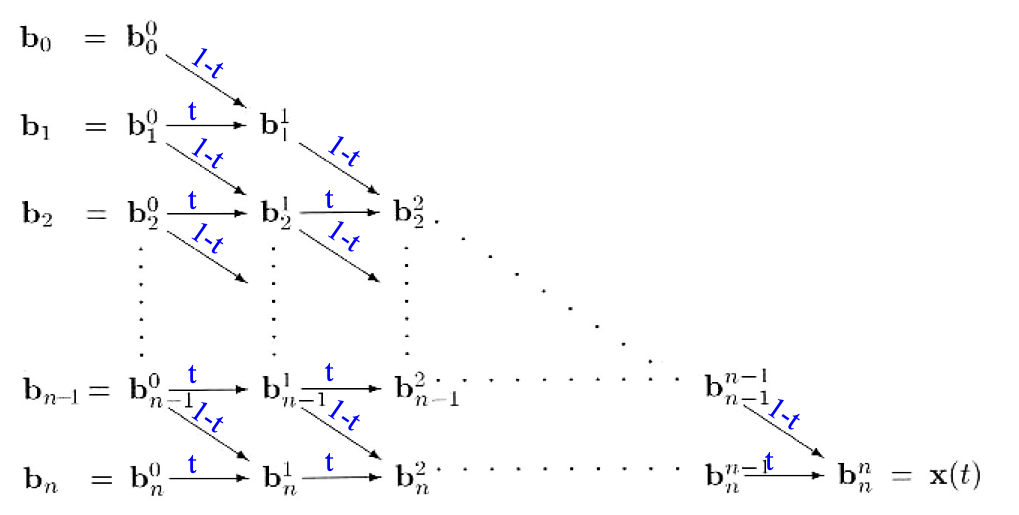
\includegraphics[scale=0.5]{images/de_Casteljau.png}
\end{center}
Durch die Methode der Subdivision mit Hilfe von de Casteljau können Kurven durch kleine Linien sehr effizient dargestellt werden

Durch Rekursion mit Startpunkt in der Mitte konvergiert de Casteljau sehr schnell
\subsection{Glatter Übergang zwischen benachbarten Kurven}
\begin{itemize}
	\item Stetigkeit falls: $b_n = c_0$
	\item Tangenten im Punkt $b_n = c_0$ sind gegeben durch
		\begin{itemize}
			\item $C'(1)=n(b_n-b_n1)$
			\item $B'(0)=n(c_1-c_0)$
		\end{itemize}
	
	Glatt, falls $b_{n-1}, b_n = c_0, c_1$ kollinear sind

\end{itemize}
\subsection{Tensor-Produkt-Bezier-Flächen}
\subsubsection{Allgemein}
$$
	F(s,t) = \sum_{k=0}^m \sum_{i=0}^n b_{ik} B_i^n(s)B_k^m(t)=\sum_{i=0}^n(\sum_{k=0}^m b_{ik} B_k^m(t))B_i^n(t)
$$
Die Kontrollpunkte hängen von $t$ ab
$$
	d_i(t) = \sum_k b_{ik} B_k^m (t)
$$
Kurven mit $s=$const sind Bezier-Kurven in $t$
$$
	F(s,t)=\sum_k c_k(s) B_k^m(t) \text{ mit } c_k(s) = \sum_i b_{ik} B_i^m (s)
$$
Alle Formeigenschaften, außer der Variationsreduktion übertragen sich von den Bezier-Kurven
\subsubsection{Auswertung}
1D Vrsion: Zurrest eindimensional in erste Richtung mit de Casteljau, dann in die andere.

Verallgemeinerung der bilinearen Interpolation: Coons-Patch
\begin{align*}
	P_1 &= C_W(0) = C_S(0) \\
	P_2 &= C_O(0) = C_S(1) \\
	P_3 &= C_N(0) = C_W(1) \\
	P_4 &= C_N(1) = C_O(1)
\end{align*} 
$$
	F_{st}(s,t)=(1-s)(1-t)P_1 + s(1-t)P_2 + (1-s)tP_3 + stP_4
$$